\documentclass[11pt]{article}
\usepackage{amsmath, amssymb, amsthm}
\usepackage[retainorgcmds]{IEEEtrantools}

\usepackage[pdftex]{graphicx}
\usepackage{tikz}
\usetikzlibrary{intersections}

\usepackage{fancyhdr}

%Listings stuff
\usepackage{listings}
\usepackage{lstautogobble}
\usepackage{color}

\definecolor{gray}{rgb}{0.5,0.5,0.5}
\lstset{
basicstyle={\small\ttfamily},
tabsize=3,
numbers=left,
numbersep=5pt,
numberstyle=\tiny\color{gray},
stepnumber=2,
breaklines=true,
boxpos=t
}

%Format stuff
\pagestyle{fancy}
\headheight 35pt

%Header info
\chead{\Large \textbf{Automata and Regex}}
\lhead{}
\rhead{}

\begin{document}
\section{Finite Automata}
	A finite automata is an abstract machine that starts in an initial state, and repeats some task until it ends up in a final state. An automata may have 0 or more end states but only a single start state. When using an automata to implement regex matching, the validity of a string is determined by whether or not the ending state of the automata after parsing is the final state.
	
	It is possible for an automata to have a \textbf{dead state}, that is a non-final state with no possibility of exiting. Most cases these dead states will be omitted from diagrams, so it is safe to assume that any nonexistant edges all lead to a dead state.
	
	\begin{center}
	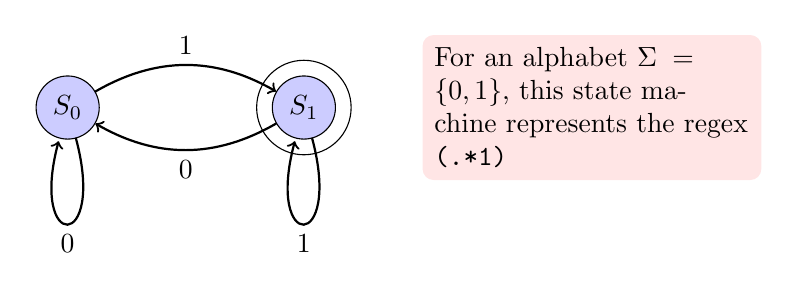
\begin{tikzpicture}
		[scale=3,line cap=round,
		%Styles
		axes/.style=,
		important line/.style={very thick},
		information text/.style={rounded corners,fill=red!10,inner sep=1ex},
		dot/.style={circle,inner sep=1pt,fill,label={#1},name=#1}	,
		main node/.style={circle,fill=blue!20,draw}		
		]
		
		%Colors
		\colorlet{anglecolor}{green!50!black}	%angle arcs/lines
		
		%The graphic
		\node[main node] (S0) at (0,0) {$S_0$};
		\node[main node] (S1) at (1, 0) {$S_1$};
		\draw (1, 0) circle (.2cm);
		
		\path 	(S0)	edge [bend left,->,thick] node[above]{$1$}	(S1)
							edge [loop below,->,thick] node[below]{$0$} (S0)
					(S1)	edge [bend left,->,thick] node[below]{$0$} (S0)
							edge [loop below,->,thick] node[below]{$1$} (S1);
							
		\draw[xshift=1.5cm]
			node[information text,right,text width=4cm] {For an alphabet $\Sigma = \{0,1\}$, this state machine represents the regex \verb|(.*1)|};
	\end{tikzpicture}
	\end{center}
	
\section{Deterministic Finite Automata}
	A DFA cannot have more than one transition leaving a state on the same symbol. A DFA will always produce the exact same path for any given string. A DFA formally is a 5-tuple $(Q, \Sigma, \delta, q_0, F)$.
	\begin{itemize}
		\item $Q$: Finite, non-empty set of states
		\item $\Sigma$: Input alphabet
		\item $\delta$: A transition function $\delta : Q\times \Sigma \rightarrow Q$
		\item $q_0$: A state state $q_0 \in Q$
		\item $F$: A set of final states $F \subset Q$
	\end{itemize}
	
\section{Nondeterministic Finite Automata}
	An NFA can have multiple multiple paths leaving a state encoded with the same symbol. An NFA will yield many possible paths for a given string, and determining the validity of a string requires a backtracking graph search. Formally, an NFA is a 5-tuple $(Q, \Sigma, \Delta, q_0, F)$ with $\Delta : Q \times \Sigma \rightarrow P(Q)$ where $P(Q)$ is the powerset of $Q$.
	
	\subparagraph{NFA-$\epsilon$} An NFA-$\epsilon$ has one or more paths encoded as an empty character, meaning that when reading through string it is possible to take a path without actually advancing a character.
	
\section{Languages}
	A language $L$ is a set of strings defined over an alphabet $\Sigma$ which is a finite set of symbols. There are three operations defined on languages:
	\begin{itemize}
		\item Concatenation: $L_1L_2 = \{xy \mid x \in L_1,  y \in L_2\}$
		\item Union: $L_1 \cup  L_2 = \{x \mid x \in L_1 \text{ or } x \in L_2\}$
		\item Kleene Closure: $L^* = \cup_{i\in N} L^i$, concatenate 0 or more strings from $L$.
	\end{itemize}
	Thus, the language $L^n$, a language consisting of n-length strings, can be built inductively as $LL^{n-1}$.
	
	\subsection{Regular Expressions}
		Regular expressions over $\Sigma$ are representations of languages, and are defined inductively as such:
		\begin{center}
		\begin{tabular}{c|c}
			Regex & Language\\\hline
			$\emptyset$ & $\emptyset$\\
			$\epsilon$ & $\{\epsilon\}$\\
			$\forall \sigma \in \Sigma$ & $\{\sigma\}$\\
			$AB$ & $L_AL_B$\\
			$(A|B)$ & $L_A \cup L_B$\\
			$A^*$ & $L_A^*$
		\end{tabular}
		\end{center}
	
		If $s \in [[RE]]$, then the string $s$ is recognized by the regular expression. The languages that can be described by regular expressions are called \textbf{regular languages}. Not all languages are regular languages, however.
		
\section{NFA Representation of Regex}
	To transform a regex into an NFA (e.g. for a regex engine), define the following two recursive predicates:
	\begin{itemize}
		\item $e\checkmark$: Holds if $\epsilon \in [[e\checkmark]]$.
	\end{itemize}

%	\begin{center}
%	\begin{tikzpicture}
%		[scale=3,line cap=round,
%		%Styles
%		axes/.style=,
%		important line/.style={very thick},
%		information text/.style={rounded corners,fill=red!10,inner sep=1ex},
%		dot/.style={circle,inner sep=1pt,fill,label={#1},name=#1}			
%		]
%		
%		%Colors
%		\colorlet{anglecolor}{green!50!black}	%angle arcs/lines
%		
%		%The graphic
%	\end{tikzpicture}
%	\end{center}

%	\begin{figure}[htb]
%		\centering
%		\includegraphics[width=0.8\textwidth]{filename.eps}
%		\caption{Caption.}
%		\label{fig:figure}
%	\end{figure}

%		\def\enotesize{\normalsize}
%		\theendnotes
\end{document}